\chapter[PROPOSTA]{PROPOSTA}
\label{chapter:architecture}

O InterSCity se encontra atualmente em um estado estável e relativamente maduro,
mas carece robustez quanto ao processamento de seus dados. Neste capítulo serão
apresentadas definições e ferramentas escolhidas para compor o processamento
de dados do InterSCity, bem como as justificativas que levaram às decisões. Ao
fim, será levantado o escopo do que deve ser desenvolvido neste trabalho.

\section{ARQUITETURA}

A arquitetura definida para o desenvolvimento da camada de processamento de
dados do InterSCity é a Arquitetura Kappa. A Arquitetura Lambda embora já seja
difundida em projetos de excelência, é demasiadamente complexa para o contexto
em questão, de modo que manter duas bases de código, grandes e complexas,
desvia de um dos focos do InterSCity, que é a manutenibilidade. Dessa forma, a
escolha pela Arquitetura Kappa parece ser a mais adequada no contexto do
InterSCity.

\section{TECNOLOGIAS}

As tecnologias definidas para a proposta foram feitas levando em conta as
seguintes prioridades:

\begin{enumerate}
    \item \textit{Software} livre;
    \item Tecnologias já usadas no InterSCity;
    \item Interoperabilidade com as tecnologias já usadas terão prioridade;
    \item Melhor manutenibilidade;
    \item Melhor escalabilidade e performance.
\end{enumerate}

Tecnologias de \textit{software} livre tiveram prioridade máxima pelo
ecossistema Big Data ser composto de ferramentas livres de alto nível, e por
ser um dos pilares do InterSCity. Tecnologias já usadas pelo InterSCity também
tiveram grande peso por não forçarem grandes mudanças ao ecossistema já
estabelecido, facilitando a aceitação da proposta por parte dos responsáveis do
InterSCity. Os outros fatores de prioridade já são focos do InterSCity,
mas foi dada prioridade a manutenibilidade no lugar da performance, pelo
contexto atual do InterSCity não apresentar grandes problemas de performance.

\begin{figure}
  \centering
    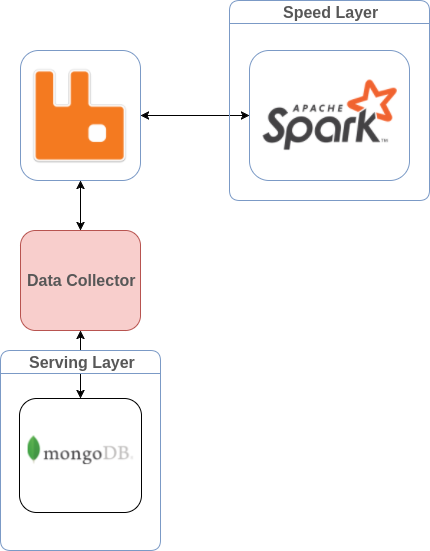
\includegraphics[scale=0.5]{figuras/stack.png}
  \caption{Pilha de tecnologias utilizadas - RabbitMQ, Apache Spark e MongoDB.}
  \label{fig:stack}
\end{figure}


\subsection{Broker}

O \textit{broker} que será utilizado para transmissão dos dados é o
\textbf{RabbitMQ}. O principal critério utilizado foi o fato dele já ser usado
pelo InterSCity, de modo que a troca para outra tecnologia não seria
interessante, além do fato da escolha não comprometer em nenhum critério.
Contudo, têm-se noção que o Kafka seria uma solução tão boa quanto, tendo ainda
performance superior ao RabbitMQ, e disponibilizando o \textit{log} de
transações, que seria de grande utilidade no desenvolvimento da Arquitetura
Kappa.

\subsection{Streaming}

A tecnologia de \textit{streaming} que será utilizada é o \textbf{Apache Spark}.
O Apache Spark, como já levantado, tem alta performance, atende bem os
requisitos, e tem suporte para várias tecnologias, como Python, R, Scala e
Java. O fator mais importante na escolha foi o diferencial de conter integrado
multiplas formas de processamento (\textit{batch} e \textit{streaming}) e
biblioteca de \textit{machine learning} que pode vir a ser útil.
Por ser tão abrangente, o Spark seria a única tecnologia necessária quanto ao
processamento de dados, seguindo assim o princípio de \textit{framework} único
da Arquitetura Kappa. Além disso, uma transição para a Arquitetura Lambda seria
fácil caso fosse de interesse do InterSCity, pelo Spark abranger as duas formas
de processamento necessárias.

\subsection{Banco de dados NoSQL}

A tecnologia de banco de dados NoSQL definida é o \textbf{MongoDB}. O principal
motivo é o fato dele já ser usado pelo InterSCity, e o fato dele não
comprometer nenhum critério. Contudo, assim como no caso do \textit{broker},
têm-se noção que o Apache Cassandra também seria uma ótima solução no contexto
do InterSCity, principalmente por ter \textit{adapters} para o Spark e para o
RabbitMQ.

\section{IMPLEMENTAÇÃO}

A implementação e contribuição deste trabalho será então uma camada de
processamentos funcional e pronta para ser utilizada, utilizando as
ferramentas citadas anteriormente. Ás mesmas abordagens utilizadas pelo
InterSCity serão seguidas (como uso do Docker), de modo que possa ser
aderido pela comunidade da plataforma sem maiores problemas. Além disso, será
desenvolvido um pequeno exemplo que utiliza a plataforma e a camada de
processamento, de modo que ilustre o uso do módulo desenvolvido, contudo, se
trata de algo ilustrativo e não um caso real de uso.
